\section{Database Comparison}\label{sec:database_comparison}
The three databases we used were overlapping but distinct. The size of these
overlaps is shown in Figure S~\ref{fig:database_overlap}.

\begin{figure}[!h]
    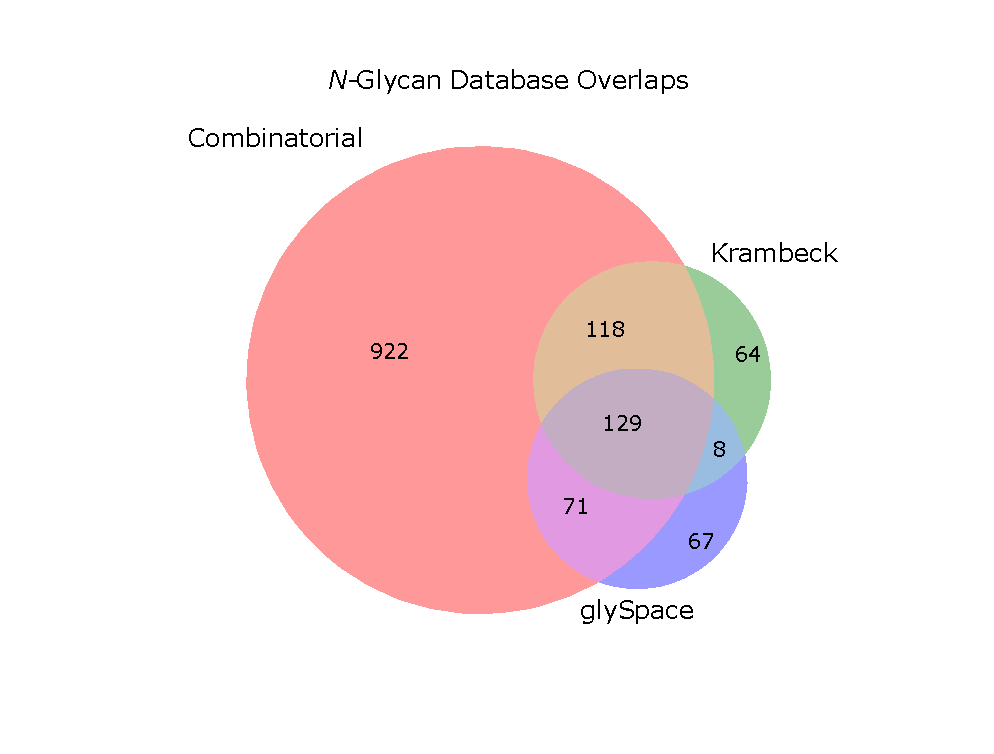
\includegraphics[width=.95\linewidth]{figure/database-venndiagram.eps}
    \caption{The overlap of the source databases used\label{fig:database_overlap}.
    As expected, the combinatorial database contains an enormous number of
    compositions not found in either other database, many of which are not
    biosynthetically feasible for humans. Those found in the Krambeck database but
    not the combinatorial or glySpace database are derived from lactosamine extensions
    run to the limit of the biosynthetic process covered in the original simulation
    (\citealp{Krambeck2005}). The glySpace database contained composition units not
    found in the other two databases, such as Xylose, Sulfate, and Phosphate.}
\end{figure}
